\documentclass[11pt,a4paper,titlepage]{article}

% --- Packages ---
\usepackage[utf8]{inputenc}
\usepackage[T1]{fontenc}
\usepackage{lmodern}
\usepackage{hyperref}
\usepackage{geometry}
\usepackage{titlesec}
\usepackage{xcolor}
\usepackage{listings}
\usepackage{graphicx}
\usepackage{fancyhdr}
\usepackage{tocloft}
\usepackage{enumitem}
\usepackage{tikz}
\usetikzlibrary{shapes.geometric, arrows, positioning}


% --- Page Layout ---
\geometry{
    margin=1in,
    headheight=14pt
}

% --- Colors ---
\definecolor{navblue}{RGB}{0, 51, 102}
\definecolor{navlight}{RGB}{0, 102, 204}
\definecolor{codebackground}{RGB}{248, 248, 248}
\definecolor{codegray}{RGB}{128, 128, 128}

% --- Hyperref Setup ---
\hypersetup{
    colorlinks=true,
    linkcolor=navblue,
    urlcolor=navlight,
    citecolor=navblue,
    pdftitle={NavHAL Technical White Paper},
    pdfauthor={NAVRobotec Pvt Ltd}
}

% --- Typography ---
\titleformat{\section}{\large\bfseries\color{navblue}}{\thesection}{1em}{}[\titlerule]
\titleformat{\subsection}{\normalsize\bfseries\color{navblue}}{\thesubsection}{1em}{}

% --- Header and Footer ---
\pagestyle{fancy}
\fancyhf{}
\lhead{\color{codegray}NavHAL: Technical White Paper}
\rhead{\color{codegray}NAVRobotec Pvt Ltd}
\cfoot{\thepage}
\renewcommand{\headrulewidth}{0.4pt}
\renewcommand{\footrulewidth}{0pt}

% --- Code Listing Style ---
\lstset{
    backgroundcolor=\color{codebackground},
    basicstyle=\ttfamily\small,
    breaklines=true,
    frame=single,
    rulecolor=\color{lightgray},
    keywordstyle=\color{blue}\bfseries,
    commentstyle=\color{codegray}\itshape,
    stringstyle=\color{red},
    numbers=left,
    numberstyle=\tiny\color{codegray},
    stepnumber=1,
    showstringspaces=false,
    captionpos=b
}

% --- Title Information ---
\title{
    \vspace{2cm}
    \includegraphics[width=0.4\textwidth]{example-image} \\ % Placeholder for logo
    \vspace{2cm}
    \textbf{\Huge \color{navblue} NavHAL} \\
    \vspace{0.5cm}
    \large \textbf{The Architecture-Agnostic Hardware Abstraction Layer} \\
    \vspace{1.5cm}
    \Large \textit{A Technical White Paper on Scalable Embedded Development} \\
    \vspace{2cm}
}

\author{
    \textbf{NAVRobotec Pvt Ltd} \\
    \small 25INS001 Research \& Development Division \\
    \small \href{mailto:support@navrobotec.com}{support@navrobotec.com} \\
    \small \url{https://navrobotec.com}
}

\date{\today}

\begin{document}

\maketitle

\begin{abstract}
NavHAL is a professional-grade, cross-platform hardware abstraction layer (HAL) designed to harmonize embedded software development across diverse hardware architectures. By decoupling high-level application logic from low-level register manipulation, NavHAL provides a consistent, efficient, and type-safe interface for modern microcontroller units (MCUs). This paper explores the design philosophy, technical architecture, and strategic roadmap of NavHAL, demonstrating its role as a critical enabler for portable and maintainable embedded systems in the fields of robotics, drones, and industrial automation.
\end{abstract}

\newpage
\tableofcontents
\newpage

% --- Sections ---
\section{Introduction}
\label{sec:introduction}

In the contemporary era of embedded engineering, the disparity between silicon capability and software scalability has never been more pronounced. As microcontrollers (MCUs) evolve to feature more complex interconnects, heterogeneous multi-core architectures, and specialized hardware accelerators, the software layers responsible for managing these resources have traditionally remained siloed within vendor-specific ecosystems. This fragmentation represents a multi-billion dollar friction point in the global electronics industry, leading to extended development cycles, high porting costs, and a significant accumulation of technical debt.

\subsection{The Landscape of Embedded Abstraction}
To understand the necessity of NavHAL, one must first analyze the current state of the market. Existing solutions generally fall into three categories, each with inherent limitations:

\begin{enumerate}
    \item \textbf{Vendor-Specific HALs (e.g., STM32CubeHAL, NXP MCUXpresso, TI DriverLib)}:
    These are the most common tools in a professional engineer's arsenal. While they provide comprehensive support for a specific vendor's silicon, they are fundamentally designed to create "sticky" ecosystems. Code written for STM32CubeHAL is virtually impossible to port to an NXP or Microchip target without a complete rewrite of the peripheral integration layer. Furthermore, these HALs are often criticized for being overly "heavy," with deep call stacks and excessive abstraction that can obscure the underlying hardware performance.

    \item \textbf{High-Level Prototyping Frameworks (e.g., Arduino, Mbed OS)}:
    Frameworks like Arduino have revolutionized accessibility but at the cost of professional rigor. The Arduino "Wire" or "Serial" APIs are designed for simplicity, not high-performance industrial applications. They often lack low-level control (e.g., precise DMA configuration or advanced timer synchronization) and introduce significant memory and execution overhead that is unacceptable in many resource-constrained or safety-critical environments.

    \item \textbf{RTOS Abstraction Layers (e.g., Zephyr RTOS, RT-Thread)}:
    Modern RTOSs like Zephyr provide impressive cross-architecture support through a unified driver model. However, these systems are "all-in" solutions. To use the Zephyr HAL, one must typically adopt the entire Zephyr build system, kernel, and philosophy. For many bare-metal projects, or for teams requiring a lightweight, modular HAL that doesn't dictate the threading model or OS structure, these platforms are often too invasive.
\end{enumerate}

\subsection{The NavHAL Differentiator: What We Did Different}
NavHAL, developed by \textbf{NAVRobotec Pvt Ltd}, was engineered from the ground up to occupy a "Professional-Agile" middle ground. Our approach differs from the industry standard in several key dimensions:

\subsubsection{Architecture-Agnostic Single-Root Dispatch}
Unlike vendor HALs that require separate projects for separate MCUs, NavHAL uses a "Single-Root" architecture. A developer can switch from an ARM Cortex-M4 (STM32) to an RP2040 or an AVR target by changing a single build flag in CMake. The application-level API (\texttt{hal\_gpio\_write}, etc.) remains identical, while the build system automatically dispatches to the correct register-level implementation.

\subsubsection{C11 Type-Polymorphism via \texttt{\_Generic}}
One of the primary frustrations with C-based HALs is the proliferation of type-specific functions (e.g., \texttt{Serial.printInt}, \texttt{Serial.printFloat}). NavHAL leverages modern C11 features, specifically \texttt{\_Generic} macros, to provide a polymorphic interface that is both type-safe and incredibly clean. As demonstrated in section \ref{sec:peripherals}, a single \texttt{uart\_write()} call can handle multiple data types without the overhead of runtime type checking or the verbosity of C++, all while remaining strictly within the domain of standard C.

\subsubsection{Zero-Invasive Bare-Metal Kernel}
NavHAL does not assume an OS. It is designed to be the foundation upon which an OS (like our own \textit{Vaios}) is built, not a byproduct of one. This allows it to be used in ultra-low-power, deterministic, bare-metal loops where every clock cycle counts, while still providing the modularity required for high-level application development.

\subsubsection{Hardware-Direct Register Maps}
To avoid the bloat of third-party libraries, NavHAL maintains its own optimized register maps. This provides us with full control over the memory layout and ensures that we are never "waiting on a vendor update" to fix a low-level driver bug. It also allows for a drastically smaller binary footprint, critical for 8-bit and 16-bit migrations.

\subsection{Vision: Bridging Man and Machine}
At \textbf{NAVRobotec}, we believe that software should be as resilient and adaptable as the hardware it controls. NavHAL is our solution to the fragmentation crisis---a tool built by engineers, for engineers, designed to make "Write Once, Run Anywhere" a reality even at the lowest levels of silicon.

\section{Technical Architecture}
\label{sec:architecture}

The architecture of NavHAL is designed to address the "Abstraction-Efficiency Paradox" in embedded systems: the need for high-level, portable APIs that does not introduce the overhead typically associated with heavyweight middleware. This is achieved through a meticulously layered design that decouples peripheral logic from hardware topology.

\subsection{The Layered Abstraction Model}
NavHAL is designed as a vertical abstraction stack that ensures hardware independence while maintaining minimal execution overhead. The architecture is organized into four logical tiers:

\begin{figure}[h]
    \centering
    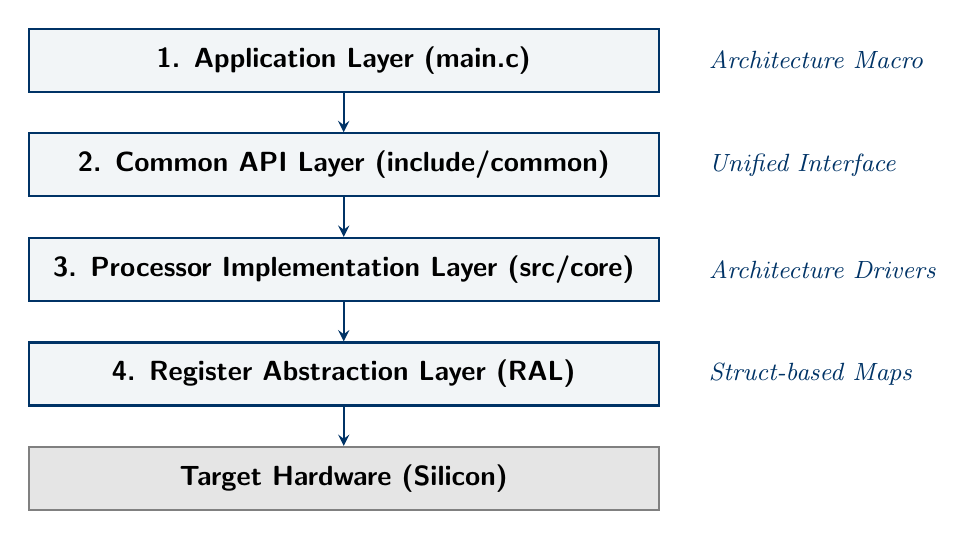
\begin{tikzpicture}[
        layer/.style={rectangle, draw=navblue, fill=navblue!5, thick, minimum width=8cm, minimum height=0.8cm, text centered, font=\sffamily\bfseries},
        arrow/.style={-stealth, thick, navblue},
        node distance=0.5cm
    ]
        % Nodes
        \node (app) [layer] {1. Application Layer (main.c)};
        \node (common) [layer, below=of app] {2. Common API Layer (include/common)};
        \node (arch) [layer, below=of common] {3. Processor Implementation Layer (src/core)};
        \node (ral) [layer, below=of arch] {4. Register Abstraction Layer (RAL)};
        \node (hw) [layer, fill=gray!20, draw=gray, below=of ral] {Target Hardware (Silicon)};

        % Arrows
        \draw [arrow] (app) -- (common);
        \draw [arrow] (common) -- (arch);
        \draw [arrow] (arch) -- (ral);
        \draw [arrow] (ral) -- (hw);

        % Annotations
        \node [right=0.5cm of app, font=\small\itshape, text=navblue] {Architecture Macro};
        \node [right=0.5cm of common, font=\small\itshape, text=navblue] {Unified Interface};
        \node [right=0.5cm of arch, font=\small\itshape, text=navblue] {Architecture Drivers};
        \node [right=0.5cm of ral, font=\small\itshape, text=navblue] {Struct-based Maps};

    \end{tikzpicture}
    \caption{The NavHAL Abstraction Stack}
    \label{fig:abstraction_stack}
\end{figure}

\begin{enumerate}
    \item \textbf{Application Layer}: The entry point where the target architecture is defined (e.g., \texttt{\#define CORTEX\_M4}) and generic HAL functions are invoked.
    \item \textbf{Common API Layer}: Architecture-agnostic headers in \texttt{include/common/} that route calls to the specific architecture implementation.
    \item \textbf{Processor Implementation Layer}: Source files in \texttt{src/core/<processor>/} that provide the actual logic for peripherals like GPIO, UART, and I2C.
    \item \textbf{Register Abstraction Layer (RAL)}: Low-level headers defining memory-mapped register structures for precise hardware control.
\end{enumerate}

\subsection{The Architecture-Led Dispatch Mechanism}
NavHAL's portability is driven by an explicit architecture selection mechanism. Instead of complex runtime auto-detection, the HAL relies on a clear, preprocessor-driven dispatch system.

\subsubsection{Explicit Architecture Selection}
Selection of the hardware target is performed at the top of the application or via build-system compiler flags. By defining a macro such as \texttt{CORTEX\_M4}, the system "activates" the corresponding low-level headers.

\subsubsection{Header Dispatch Logic}
The headers in the \texttt{include/common/} directory act as the primary dispatchers. They check for defined architecture macros and include the relevant sub-headers from the \texttt{include/core/} directory.

\begin{figure}[h]
    \centering
    \begin{tikzpicture}[
        node/.style={rectangle, draw=navblue, fill=navblue!5, thick, text centered, font=\sffamily\small},
        decision/.style={diamond, draw=navblue, fill=orange!10, thick, text centered, inner sep=0pt, font=\sffamily\tiny, width=2.5cm},
        arrow/.style={-stealth, thick, navblue}
    ]
        % Nodes
        \node (app) [node] {Application (\texttt{main.c})};
        \node (def) [node, below=0.8cm of app, fill=green!5] {\texttt{\#define CORTEX\_M4}};
        \node (common) [node, below=0.8cm of def] {\texttt{include/common/hal\_gpio.h}};
        \node (dispatch) [decision, below=1.0cm of common] {\texttt{if CORTEX\_M4}};
        \node (impl) [node, right=1.5cm of dispatch] {\texttt{include/core/cortex-m4/gpio.h}};

        % Arrows
        \draw [arrow] (app) -- (def);
        \draw [arrow] (def) -- (common);
        \draw [arrow] (common) -- (dispatch);
        \draw [arrow] (dispatch) -- node[above, font=\tiny] {Yes} (impl);

    \end{tikzpicture}
    \caption{Preprocessing Dispatch Flow}
    \label{fig:dispatch_flow}
\end{figure}

\subsubsection{Source File Selection via CMake}
While the headers are dispatched via the preprocessor, the source files are selected by the CMake build system. The root \texttt{CMakeLists.txt} uses the \texttt{CMAKE\_SYSTEM\_PROCESSOR} variable to include the appropriate implementation directory within \texttt{src/core/}. 

This dual-mechanism ensures that only the necessary code is included in the project, fulfilling the \textit{Zero-Cost Abstraction} principle: the hardware-specific implementation is effectively "linked" directly to the common API calls without intermediate layers or runtime overhead.

\subsection{Directory Structure and Organization}
The project follows a strict hierarchical layout to ensure scalability:
\begin{itemize}
    \item \textbf{\texttt{include/common/}}: Architecture-independent API headers.
    \item \textbf{\texttt{include/core/<processor>/}}: Hardware-specific register maps and function prototypes.
    \item \textbf{\texttt{src/core/<processor>/}}: Implementation logic grouped by peripheral (GPIO, UART, etc.).
    \item \textbf{\texttt{src/board/<board>/}}: Board-specific files such as linker scripts and system configuration.
\end{itemize}

\subsection{Registry Abstraction: The Structure-Based Approach}
Unlike many HALs that rely on a sea of \texttt{\#define} constants for register offsets, NavHAL employs a structure-based mapping system. Each peripheral is represented as a packed C \texttt{struct}, where the members correspond to specific hardware registers at precise memory offsets.

\begin{lstlisting}[language=C, caption=GPIO Register Mapping (Cortex-M4)]
typedef struct {
  __IO uint32_t MODER;   /* Mode register */
  __IO uint32_t OTYPER;  /* Output type register */
  __IO uint32_t OSPEEDR; /* Output speed register */
  __IO uint32_t PUPDR;   /* Pull-up/pull-down register */
  /* ... Additional registers ... */
} GPIOx_Typedef;

#define GPIOA_BASE_ADDR 0x40020000
#define GPIOA ((GPIOx_Typedef *)GPIOA_BASE_ADDR)
\end{lstlisting}

This methodology provides several advantages:
\begin{itemize}
    \item \textbf{Type Safety}: Prevents accidental writes to incorrect memory locations by providing structured access.
    \item \textbf{Readability}: Allows code like \texttt{GPIOA->MODER = 0x1;} which is far more intuitive than complex bitwise offset arithmetic.
    \item \textbf{Debuggability}: Modern debuggers (GDB/Ozone) can naturally parse these structures, allowing for real-time inspection of peripheral states in a human-readable format.
\end{itemize}

\subsection{Memory Topology and Port Mapping}
To maintain a unified API for heterogeneous hardware, NavHAL uses an "Absolute Pin Mapping" system. A single integer or enum defines a pin (e.g., \texttt{PA5}), and the HAL provides macros to compute the corresponding port structure and pin offset at compile or runtime.

\begin{lstlisting}[language=C, caption=Port Resolution Macro]
#define GPIO_GET_PORT(pin) ((GPIOx_Typedef *)(GPIOA_BASE_ADDR + ((pin / 16) * 0x400)))
#define GPIO_GET_PIN_OFFSET(pin) (pin % 16)
\end{lstlisting}

This abstraction allows for high-level functions like \texttt{hal\_gpio\_digitalwrite(PA5, HIGH)} to remain consistent across different chip families, even when the underlying port counts or memory layouts differ.

\subsection{Modular Core Separation}
The project directory structure mirrors this architectural philosophy, ensuring that adding support for a new architecture does not require modification of existing core logic:

\begin{itemize}
    \item \texttt{include/common/}: Universal interfaces.
    \item \texttt{include/core/<arch>/}: Architecture-specific definitions.
    \item \texttt{src/core/<arch>/<peripheral>/}: Implementation of the HAL for that architecture.
\end{itemize}

By enforcing this strict modularity, NavHAL prevents "cross-pollution" between targets, keeping the codebase clean and maintainable as the number of supported MCUs grows.

\section{Peripheral Subsystems}
\label{sec:peripherals}

NavHAL provides a comprehensive suite of peripheral drivers, each engineered with a focus on ease-of-use, performance, and hardware independence. By leveraging modern C features and efficient memory-mapped I/O techniques, NavHAL offers a premium developer experience comparable to high-level frameworks but with the efficiency of bare-metal code.

\subsection{GPIO: The Universal Pin Interface}
The GPIO subsystem is the foundation of NavHAL's interaction with the physical world. It abstracts pins into a unified format (e.g., \texttt{GPIO\_PA05}) while providing granular control over electrical characteristics.

\subsubsection{Key Features}
\begin{itemize}
    \item \textbf{Mode Management}: Simple API for switching between Input, Output, Alternate Function, and Analog modes.
    \item \textbf{Electrical Configuration}: Support for internal Pull-Up/Pull-Down (PUPD) resistors, Output Type (Push-Pull vs. Open-Drain), and configurable Slew Rates.
    \item \textbf{Type-Safe Pin Mapping}: Pins are represented as unique identifiers, preventing port-mismatch errors during configuration.
\end{itemize}

\begin{lstlisting}[language=C, caption=GPIO Initialization and Control]
hal_gpio_setmode(GPIO_PA05, GPIO_OUTPUT, GPIO_PUPD_NONE);
hal_gpio_digitalwrite(GPIO_PA05, GPIO_HIGH);
\end{lstlisting}

\subsection{UART: High-Performance Serial Communication}
The UART module in NavHAL is a standout feature, offering advanced abstractions that simplify complex serial protocols.

\subsubsection{Type-Generic Write Macros}
One of NavHAL's most powerful features is the use of the C11 \texttt{\_Generic} keyword to provide a unified \texttt{write} interface. The \texttt{uart\_write()} macros automatically select the correct internal function based on the data type passed (char, int, float, or string).

\begin{lstlisting}[language=C, caption=Type-Generic UART Transmission]
uart2_write("Temperature: "); 
uart2_write(25.5f);           // Automatically calls uart2_write_float
uart2_write('\n');            // Automatically calls uart2_write_char
\end{lstlisting}

\subsubsection{DMA Integration}
For data-intensive applications, NavHAL provides a seamless path to hardware-accelerated communication. The UART driver includes built-in support for Direct Memory Access (DMA), allowing background transmissions and circular-buffer reception that offloads the CPU entirely.

\subsection{I2C and SPI: Synchronous Bus Abstractions}
The synchronous communication modules (I2C and SPI) follow a consistent transaction-based model.

\begin{itemize}
    \item \textbf{I2C Controller}: Supports Master/Slave modes, multi-byte transactions, and integrated DMA for high-bandwidth sensor data retrieval.
    \item \textbf{SPI Interface}: High-speed full-duplex communication with configurable CPOL/CPHA settings, ideal for driving displays and external storage modules.
\end{itemize}

\subsection{Timers and Pulse Width Modulation (PWM)}
NavHAL abstracts the complex timer hardware into two primary services:
\begin{enumerate}
    \item \textbf{Timebase Services}: Provides precise delays and periodic interrupts via the Systick or hardware timers.
    \item \textbf{PWM Engine}: Simplifies signal generation for motor control, LED dimming, and audio applications with an intuitive \texttt{hal\_pwm\_set\_duty()} API.
\end{enumerate}

\subsection{DMA Controller: The Performance Backbone}
The Direct Memory Access (DMA) subsystem is a critical component of NavHAL's high-performance architecture. It acts as a transparent data mover between peripherals and memory, ensuring that data-heavy tasks (like UART logging or sensor polling) do not stall the main execution thread. NavHAL's DMA management includes:
\begin{itemize}
    \item \textbf{Channel Mapping}: Automatic resolution of DMA streams and channels for supported peripherals.
    \item \textbf{Interrupt Integration}: Optional callback support for completion and error events.
\end{itemize}

\section{Hardware Implementation and Support}
\label{sec:hardware}

NavHAL is designed to be battle-tested on real-world hardware. The current implementation provides first-class support for several popular MCU families.

\subsection{STM32 Series (ARM Cortex-M4)}
The STM32 implementation is the most mature, featuring:
\begin{itemize}
    \item Full register-level abstraction for GPIO, UART, and RCC.
    \item Support for the STM32F4 series, including the ubiquitous F401RE (Nucleo-64).
    \item Hybrid approach: Direct register access for performance-critical paths and LL/HAL wrappers for complex peripherals like USB or Ethernet.
\end{itemize}

\subsection{RP2040 (Raspberry Pi Pico)}
NavHAL provides a lightweight wrapper for the RP2040's unique dual-core architecture and PIO (Programmable I/O) blocks, allowing it to fit seamlessly into the NavHAL ecosystem.

\subsection{AVR ATmega Series}
For 8-bit applications where resource constraints are paramount, NavHAL's AVR implementation focuses on ultra-low memory overhead while maintaining API compatibility with its 32-bit counterparts.

\subsection{Unified Build System: CMake}
NavHAL uses CMake as its primary build system, enabling:
\begin{itemize}
    \item \textbf{Cross-Compilation}: Easy switching between ARM-GCC, AVR-GCC, and other toolchains.
    \item \textbf{Sample-Based Workflow}: A "samples" directory allowing developers to quickly test features (e.g., \texttt{-DSAMPLE=hal\_uart}).
    \item \textbf{Integration}: Seamlessly integrates with CI/CD pipelines (GitHub Actions) for automated testing.
\end{itemize}

\section{Future Roadmap}
\label{sec:roadmap}

The evolution of NavHAL is driven by the needs of modern embedded engineering. Our roadmap focuses on several key areas of growth:

\subsection{NavHAL++ (C++ Wrapper Layer)}
To cater to the growing popularity of C++ in embedded systems, we are developing a header-only C++ wrapper layer. This will provide:
\begin{itemize}
    \item Object-oriented peripheral management.
    \item Template-based type safety for register configurations.
    \item Support for RAII (Resource Acquisition Is Initialization) for power management.
\end{itemize}

\subsection{RTOS Ecosystem Integration}
Future versions of NavHAL will include "RTOS Ports" for popular kernels like FreeRTOS, Zephyr, and RT-Thread. This includes thread-safe peripheral access and standardized OS-abstraction layers.

\subsection{Automated Hardware Testing}
We are expanding our testing suite to include "Hardware-in-the-loop" (HIL) testing, ensuring that every commit is verified on actual silicon before being merged.

\section{Conclusion}
NavHAL is more than just a library; it is a fundamental shift in how embedded software is architected. By providing a robust, high-performance, and truly portable abstraction layer, NavHAL empowers engineering teams to focus on innovation rather than hardware minutiae.

As \textbf{NAVRobotec Pvt Ltd} continues to expand the NavHAL ecosystem, it remains committed to the mission of creating seamless integration between human ingenuity and machine capability.

\vfill
\begin{center}
    \textbf{NAVRobotec Pvt Ltd} \\
    Building the Future of Embedded Systems.
\end{center}


\end{document}
